\documentclass{projectreport}

\title{Project title}
\date{Aug 20, 2022}

\coursecode{ENGG 102}
\y{I} % Year
\sem{II} % Semester/Part
\group{Computer Engineering} % Computer Science/Engineering

\member{Name 1}{Roll}
\member{Name 2}{Roll}
\member{Name 3}{Roll}
%\member{Name 4}{Roll}
%\member{Name 5}{Roll}

\supervisor{Supervisor's name}{Supervisor's academic title}{Supervisor's department}


\coordinator{Coordinator's Name}

% For abbreviations/Acronyms
\usepackage{glossaries}
\loadglsentries{glossaries}
\makenoidxglossaries

\begin{document}
	\maketitle
	
	\begin{abstract}
		It should include summary of your project work. It should answer three main questions. What are you doing? Why are you doing? And How are you doing? The abstract should cover exact problem and how your work is going to address those issues. Abstract provides description about the project in minimum possible words. Abstract should contain 150-200 words as follows:
		
		\begin{itemize}
			\item Background (1 to 2 sentences)
			\item Purpose/Aim (1 to 2 sentences)
			\item Procedure and Method/Tools (1 to 2 sentences)
			\item Expected outcome (1 to 2 sentences)
			\item Conclusion (1 sentence)
			\item Recommendation (1 sentence)
		\end{itemize}
		
	\end{abstract}

	\begin{keywords}
		Keyword1, Keyword2
	\end{keywords}

	\pagenumbering{roman}
	\setcounter{page}{1}
		
	\tableofcontents
	\listoffigures
	\listoftables
	
	\clearpage
	\printnoidxglossary[ title=Abbreviations]
	
	
	\chapter{Introduction}
	\pagenumbering{arabic}
	\setcounter{page}{1}
	This chapter introduces the proposed system. It is an elaborated form of Abstract, and is usually divided into subsections, such as background, objectives, motivation, and significance of the project.
	
	\section{Background}
	It should include basic information in the field of project work. Recent trends and development on the area of the project should be briefly discussed in this topic. It should contain at least 2-3 paragraphs, having 200-400 words.
	It should include:
	
	\begin{itemize}
		\item Recent development in the field
		\item Drawbacks and significance of existing works
	\end{itemize}
	
	\section{Objectives}
	What is the basic purpose of your project? List the objectives of your project work in bullets (not exceeding 4).
	
	\section{Motivation and Significance}
	Motivation to choose the topic, importance and contribution of your project work is included in this section.
	
	\begin{itemize}
		\item Why did you choose this particular topic as your project?
		\item How does the work address drawback of the existing systems?
		\item How is it different from the existing works?
	\end{itemize}

	It consists of a short paragraph about features of your project work. A brief introduction of features that project is going to address, helps to make the project proposal more robust.
	
	\section{Expected Outcomes}
	What outcomes do you expect from this project?
	
	\chapter{Related Works}
	
	It focuses on the discussion of similar types of other tasks/projects that have been performed earlier. It should include recent projects, works, websites, etc. as reference. Referencing should be in APA format. Below are some examples:
	
	According to \cite{doe2012}, Management Systems should include components of ...
	
	
	Thapa and Shrestha (2010) have done similar projects where they have implemented ...
	
	The Minesweeper \cite{rai2012} has features like ...
	
	Similar kinds of project work were performed earlier which have properties ...
	
	
	
	In writing this section, your purpose is to convey to your readers what knowledge and ideas have been established on a topic, and what their strengths and weaknesses are (\cite{taylor2008literature}). It should also include previous works, comparison between works, drawbacks and current works.
	
	
	\chapter{ Procedure and Methods  }
	It includes the explanation of the sequential procedure that you intend to perform during the project work. It may include algorithms, flowcharts, System Diagrams and other analysis and design which give general idea about how you approach different development procedures during the project work. It may contain a few paragraphs and diagrams which may describe your work. 
	
	
	\chapter{System Requirement Specifications}
	
	This chapter specifies the requirements of the proposed system. It may include software specifications and hardware specifications.
	
	\subsection{Software Specifications}
	This section presents the description of the proposed software system. It should include the functional and non-functional requirements of the software. It may also include software dependencies.
	
	Figure \ref{fig:usecase}\footnote{https://en.wikipedia.org/wiki/Use\_case} is an example of a use-case diagram. Table \ref{table:sample} is an example of a table.
	
	\begin{figure}[h!]
		\centering
		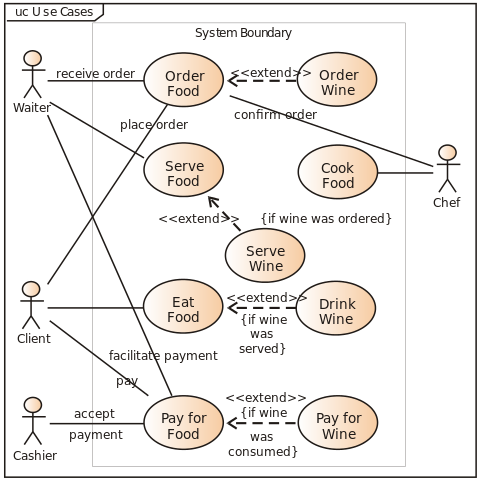
\includegraphics[width=0.8\textwidth]{usecase}
		\caption{A sample use-case diagram}
		\label{fig:usecase}
	\end{figure}

	\begin{table}[h!]
		\caption{A sample table}
		\label{table:sample}
		\centering
		\begin{tabular}{|l|l|l|}
			\hline
			\textbf{Header} & \textbf{Header} & \textbf{Header}\\ \hline
			Content & Content & Content \\ \hline
		\end{tabular}
	\end{table}
	
	\subsection{Hardware Specifications}
	It contains description of any additional hardware that may be required for the project. It also gives information about required minimum configuration of the system to develop the system.
	
	
	\chapter{Project Planning and Scheduling}
	It should give general idea on how you are planning to allocate your time/resources for different process of your project development.
	
	A Gantt chart showing the project activities and milestones is included in this section. A Gantt chart is essential to represent your time allocation for the project.
	
	A Gantt chart is a type of bar chart that illustrates a project schedule. Gantt charts illustrate the start and finish dates of the terminal elements and summary elements of a project. Terminal elements and summary elements comprise the work breakdown structure of the project.
	
	\begin{figure}[h!]
		\centering
		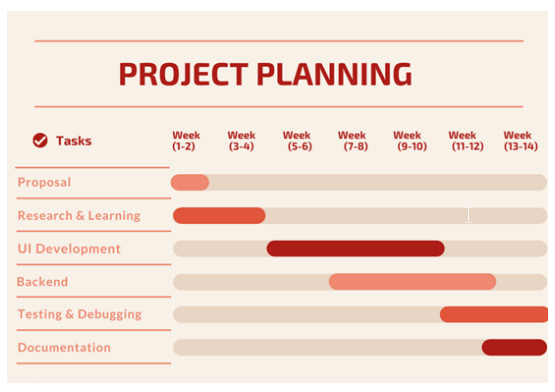
\includegraphics[width=0.8\textwidth]{gantt}
		\caption{A sample Gantt chart}
		\label{fig:gantt}
	\end{figure}

	\section{Tasks}
	
	Explain the tasks to be done to complete the project. 
	
	\begin{enumerate}
		\item Problem identification and requirement gathering
		\item Problem analysis
		\item Design 
		\item ...
	\end{enumerate}
	
	
	
	\bibliography{report}
	
	
\end{document}